\documentclass[]{article}
\usepackage{lmodern}
\usepackage{amssymb,amsmath}
\usepackage{ifxetex,ifluatex}
\usepackage{fixltx2e} % provides \textsubscript
\ifnum 0\ifxetex 1\fi\ifluatex 1\fi=0 % if pdftex
  \usepackage[T1]{fontenc}
  \usepackage[utf8]{inputenc}
\else % if luatex or xelatex
  \ifxetex
    \usepackage{mathspec}
  \else
    \usepackage{fontspec}
  \fi
  \defaultfontfeatures{Ligatures=TeX,Scale=MatchLowercase}
\fi
% use upquote if available, for straight quotes in verbatim environments
\IfFileExists{upquote.sty}{\usepackage{upquote}}{}
% use microtype if available
\IfFileExists{microtype.sty}{%
\usepackage{microtype}
\UseMicrotypeSet[protrusion]{basicmath} % disable protrusion for tt fonts
}{}
\usepackage[margin=1in]{geometry}
\usepackage{hyperref}
\hypersetup{unicode=true,
            pdftitle={Multiple Testing in Neuroscience},
            pdfauthor={Livio Finos},
            pdfborder={0 0 0},
            breaklinks=true}
\urlstyle{same}  % don't use monospace font for urls
\usepackage{graphicx,grffile}
\makeatletter
\def\maxwidth{\ifdim\Gin@nat@width>\linewidth\linewidth\else\Gin@nat@width\fi}
\def\maxheight{\ifdim\Gin@nat@height>\textheight\textheight\else\Gin@nat@height\fi}
\makeatother
% Scale images if necessary, so that they will not overflow the page
% margins by default, and it is still possible to overwrite the defaults
% using explicit options in \includegraphics[width, height, ...]{}
\setkeys{Gin}{width=\maxwidth,height=\maxheight,keepaspectratio}
\IfFileExists{parskip.sty}{%
\usepackage{parskip}
}{% else
\setlength{\parindent}{0pt}
\setlength{\parskip}{6pt plus 2pt minus 1pt}
}
\setlength{\emergencystretch}{3em}  % prevent overfull lines
\providecommand{\tightlist}{%
  \setlength{\itemsep}{0pt}\setlength{\parskip}{0pt}}
\setcounter{secnumdepth}{5}
% Redefines (sub)paragraphs to behave more like sections
\ifx\paragraph\undefined\else
\let\oldparagraph\paragraph
\renewcommand{\paragraph}[1]{\oldparagraph{#1}\mbox{}}
\fi
\ifx\subparagraph\undefined\else
\let\oldsubparagraph\subparagraph
\renewcommand{\subparagraph}[1]{\oldsubparagraph{#1}\mbox{}}
\fi

%%% Use protect on footnotes to avoid problems with footnotes in titles
\let\rmarkdownfootnote\footnote%
\def\footnote{\protect\rmarkdownfootnote}

%%% Change title format to be more compact
\usepackage{titling}

% Create subtitle command for use in maketitle
\newcommand{\subtitle}[1]{
  \posttitle{
    \begin{center}\large#1\end{center}
    }
}

\setlength{\droptitle}{-2em}

  \title{Multiple Testing in Neuroscience}
    \pretitle{\vspace{\droptitle}\centering\huge}
  \posttitle{\par}
  \subtitle{Bonferroni and Random Field Theory}
  \author{Livio Finos}
    \preauthor{\centering\large\emph}
  \postauthor{\par}
      \predate{\centering\large\emph}
  \postdate{\par}
    \date{15 Novembre 2018}


\begin{document}
\maketitle

{
\setcounter{tocdepth}{2}
\tableofcontents
}
\section{Introduction}\label{introduction}

\subsection{Biblio}\label{biblio}

\begin{itemize}
\tightlist
\item
  J Ashburner, K Friston, W Penny (2003) Human Brain Function - 2nd Ed.
  Academic Press (preprint online:
  \url{https://www.fil.ion.ucl.ac.uk/spm/doc/books/hbf2/})

  \begin{itemize}
  \tightlist
  \item
    {[}SPM14{]} Chapter 14: An introduction to Random Field Theory.
    Brett M., Penny W. and Keibel S.
  \item
    {[}SPM15{]} Chapter 15: Developments in Random Field Theory. K.J.
    Worsley
  \end{itemize}
\item
  {[}L{]} Lazar, Nicole A. (2008) The statistical analysis of functional
  MRI data. Springer
\item
  {[}PMN{]} Russell A. Poldrack, Jeanette A. Mumford, Thomas E. Nichols.
  (2011) Handbook of functional MRI data analysis. Cambridge
\item
  Friston, Holmes, Polin, Price and Frith (1996). Detecting Activations
  in PET and fMRI: Levels of Inference and Power. Neuorimage
\item
  Goeman \& Solari (2014) Tutorial in biostatistics: multiple hypothesis
  testing in genomics. Statistics in medicine
\end{itemize}

\begin{center}\rule{0.5\linewidth}{\linethickness}\end{center}

\begin{itemize}
\tightlist
\item
  MRC - Cambridge University:
  \url{http://imaging.mrc-cbu.cam.ac.uk/imaging/PrinciplesRandomFields}
\item
  wiki \url{http://en.wikipedia.org/wiki/Random_field}
\end{itemize}

The following material is largerly borrowed by:

\begin{itemize}
\tightlist
\item
  \url{https://warwick.ac.uk/fac/sci/statistics/staff/academic-research/nichols/presentations/ohbm2012/Nichols_Thresholding.pdf}
  (New and best-practice approaches to thresholding. by T. Nichols)
\item
  \url{https://fsl.fmrib.ox.ac.uk/fslcourse/lectures/feat2_part2.pdf}
  (FSL Course by FSL Group)
\item
  \url{http://www.sbirc.ed.ac.uk/cyril/SPM-course/Talks/2015/10_multiple\%20testing.pdf}
  (Cyril Pernet)
\end{itemize}

\subsection{Thresholding}\label{thresholding}

\begin{center}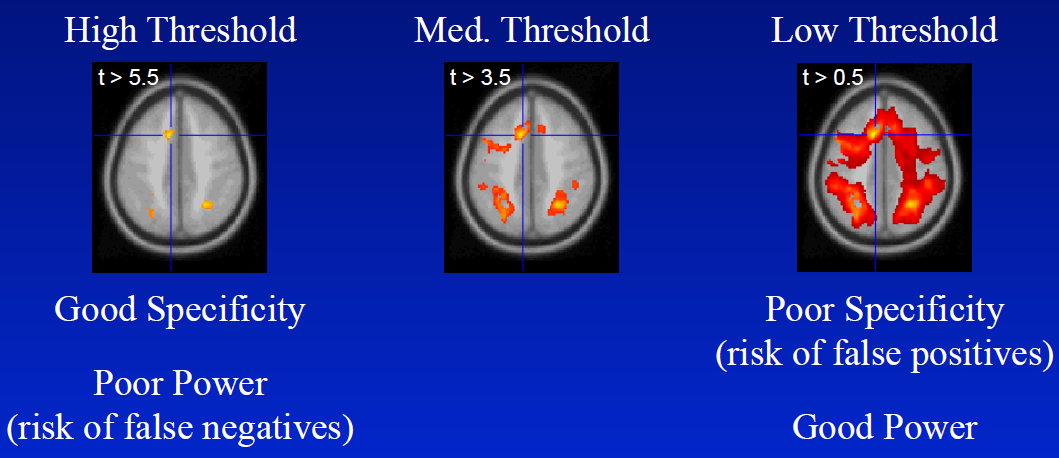
\includegraphics[width=700px]{./figs/thresolding} \end{center}

\subsection{Motivation}\label{motivation}

\begin{figure}

{\centering 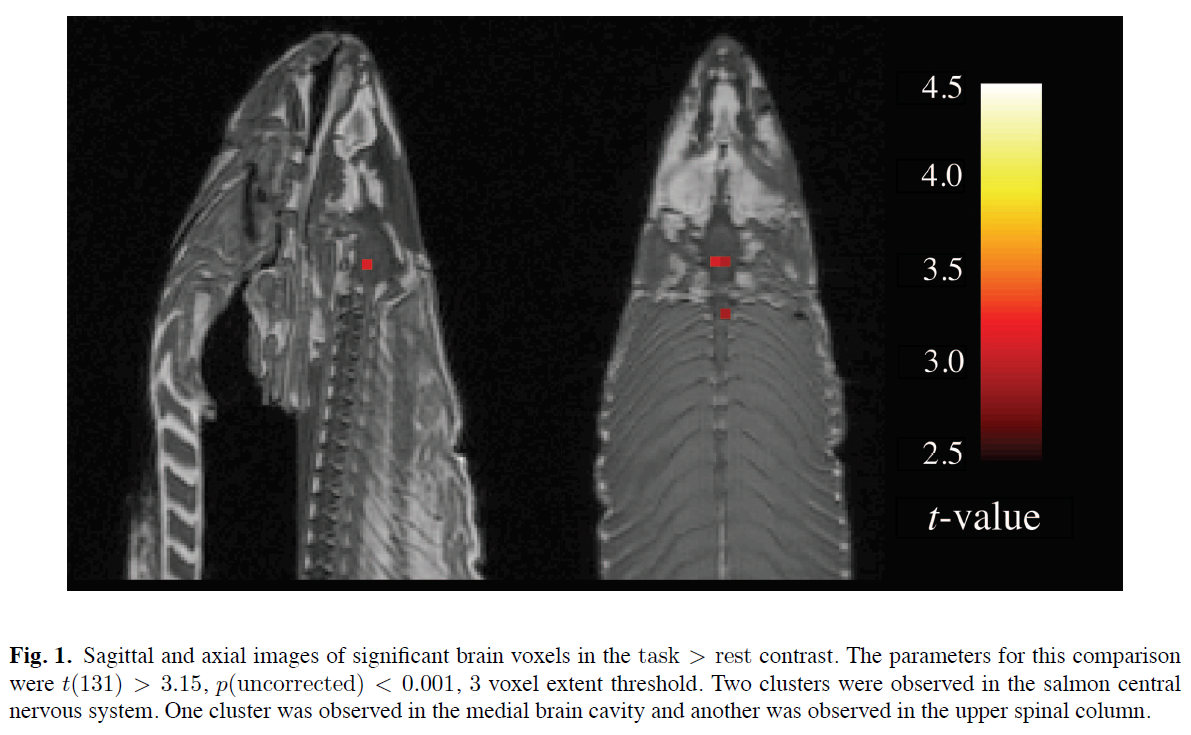
\includegraphics[width=700px]{./figs/salmon} 

}

\caption{Bennett et al. (2012)}\label{fig:unnamed-chunk-2}
\end{figure}

We need a method that ensure a given (good) Specificity and as much
Power it can.

\section{FamilyWise Error Rate}\label{familywise-error-rate}

\subsection{FamilyWise Error Rate
(FWER)}\label{familywise-error-rate-fwer}

\textbf{Probability of AT LEAST one false rejection}

\[
\begin{aligned}
    \mathrm{FWER} =\alpha &= P \big(p_i \leq \widetilde{\alpha}\ \textrm{for at least one true null hypothesis} \big) \\
    &= \mathrm{P} \Big( \bigcup_{i\in \{true\ null\ hypos\}} \{p_i \leq \widetilde{\alpha}\} \Big) \\
\end{aligned}
\]

Procedure:

\begin{itemize}
\tightlist
\item
  Fix \(\alpha\) (usually \(\alpha=.05\) or \(.01\))
\item
  Compute \(\widetilde{\alpha}\)
\item
  Derive the threshold \(u\) from \(\widetilde{\alpha}\) (e.g.~for
  \(z\)-scores:
  \(u_{\widetilde{\alpha}}=\Phi^{-1}(1-\widetilde{\alpha})\))
\end{itemize}

\subsection{Sidak Correction}\label{sidak-correction}

If one want to control (the probability of) \(FWER\) at level
\(\alpha\), what is the the \(\widetilde{\alpha}\)-level to be used for
each test?

When the \(m\) tests are \textbf{independent} (or with some form
positive dependence):

\[
\begin{aligned}
    \mathrm{FWER}= \alpha &= P \big(p_i \leq \widetilde{\alpha}\ for\ at\ least\ one\ true\ null\ hypo \big) = \\
    &= \mathrm{P} \Big( \bigcup_{i\in \{true\ null\ hypos\}} \{p_i \leq \widetilde{\alpha}\} \Big) =\\
    &= 1 - \mathrm{P} \Big( \bigcap_{i\in \{true\ null\ hypos\}} \{p_i > \widetilde{\alpha}\} \Big) = \\
    & (de Morgan)\\
    &= 1 - (1- \widetilde{\alpha})^{m_0}\ \ (m_0= \textrm{numb of true null hypos}) \\
    & (\textrm{we don't know $m_0$, but we know that $m_0\leq m$})\\
    &\leq 1 - (1- \widetilde{\alpha})^{m} 
\end{aligned}
\]

\subsection{Sidak Correction}\label{sidak-correction-1}

Hence:

\[
\begin{aligned}
    1- \alpha &= (1- \widetilde{\alpha})^{m} \\
    (1- \alpha)^{1/m} &= (1- \widetilde{\alpha}) \\
  \widetilde{\alpha} &= 1- (1- \alpha)^{1/m} 
\end{aligned}
\]

So, we define \(\widetilde{\alpha} = 1- (1- \alpha)^{1/m}\)

Declare Active all voxles with statistic
\(z \geq u_{\widetilde{\alpha}}\) (\(m =\) number of hypotheses)

Unfortunately, this solution is valid only when the p-values are
INDEPENDENT (or have a positive dependence).

In most cases, tests have a dependence induced by the original
variables.

\subsection{Bonferroni}\label{bonferroni}

\textbf{FWER}: Probability of AT LEAST one false rejection:

\textbf{Bonferroni}: \(\widetilde{\alpha} = \alpha/m\)

Declare Active all voxles with statistic
\(z \geq u_{\widetilde{\alpha}}\) (\(m =\) number of hypotheses)

FWER under control:

\[
\begin{aligned}
\mathrm{FWER} & =  P \big (p_i \leq \alpha / m \textrm{ for at least one True null hypo} \big) \\
& =  P \Big (\bigcup_{i \in \{\textrm{true null hypotheses}\}} \{p_i \leq \alpha / m \} \Big) \\
& \leq  \sum_{i \in \{\textrm{true null hypotheses}\}} \mathrm{P} (p_i \leq \alpha / m) \\
& \leq \#\{\textrm{true null hypotheses} \} \frac{\alpha}{m} \leq \alpha
\end{aligned}
\]

\begin{center}\rule{0.5\linewidth}{\linethickness}\end{center}

\textbf{Pros}

\begin{itemize}
\tightlist
\item
  Very easy
\item
  Control the FWER under any dependence
\end{itemize}

\textbf{Cons}

\begin{itemize}
\tightlist
\item
  Conservative (Adj. P-values very high, few rejections)
\end{itemize}

\section{False Discovery Rate}\label{false-discovery-rate}

\subsection{False Discovery Rate (FDR)}\label{false-discovery-rate-fdr}

\begin{center}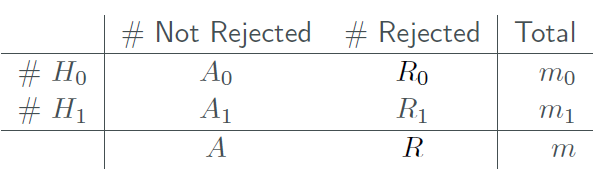
\includegraphics[width=400]{./figs/confusion} \end{center}

To control the \textbf{False Discovery Rate (FDR)} means defining a
procedure s.t.
\[ \textrm{mean}( \frac{\#  False\ Rej.s}{\# Rej.s} ) = \textrm{mean}({\frac{R_0}{R}} ) \leq \alpha\]

usually \(\alpha=.05\)

Remark: \(FWER= P({\frac{R_0}{R}}>0 ) \leq \alpha\)

\emph{Benjamini and Hochberg (1995). Journal of the Royal Statistical
Society, Series B (Methodological) 57 (1): 289--300.}

\subsection{BH procedure}\label{bh-procedure}

\begin{itemize}
\tightlist
\item
  Find the largest sorted p-value such that
  \(p_{(k)} \leq \frac{k}{m}\alpha\) (\(m =\) number of hypotheses)
\item
  Define \(\widetilde{\alpha} = p_{(k)}\)
\item
  Declare Active all voxles with statistic
  \(z \geq u_{\widetilde{\alpha}}\)
\end{itemize}

\begin{center}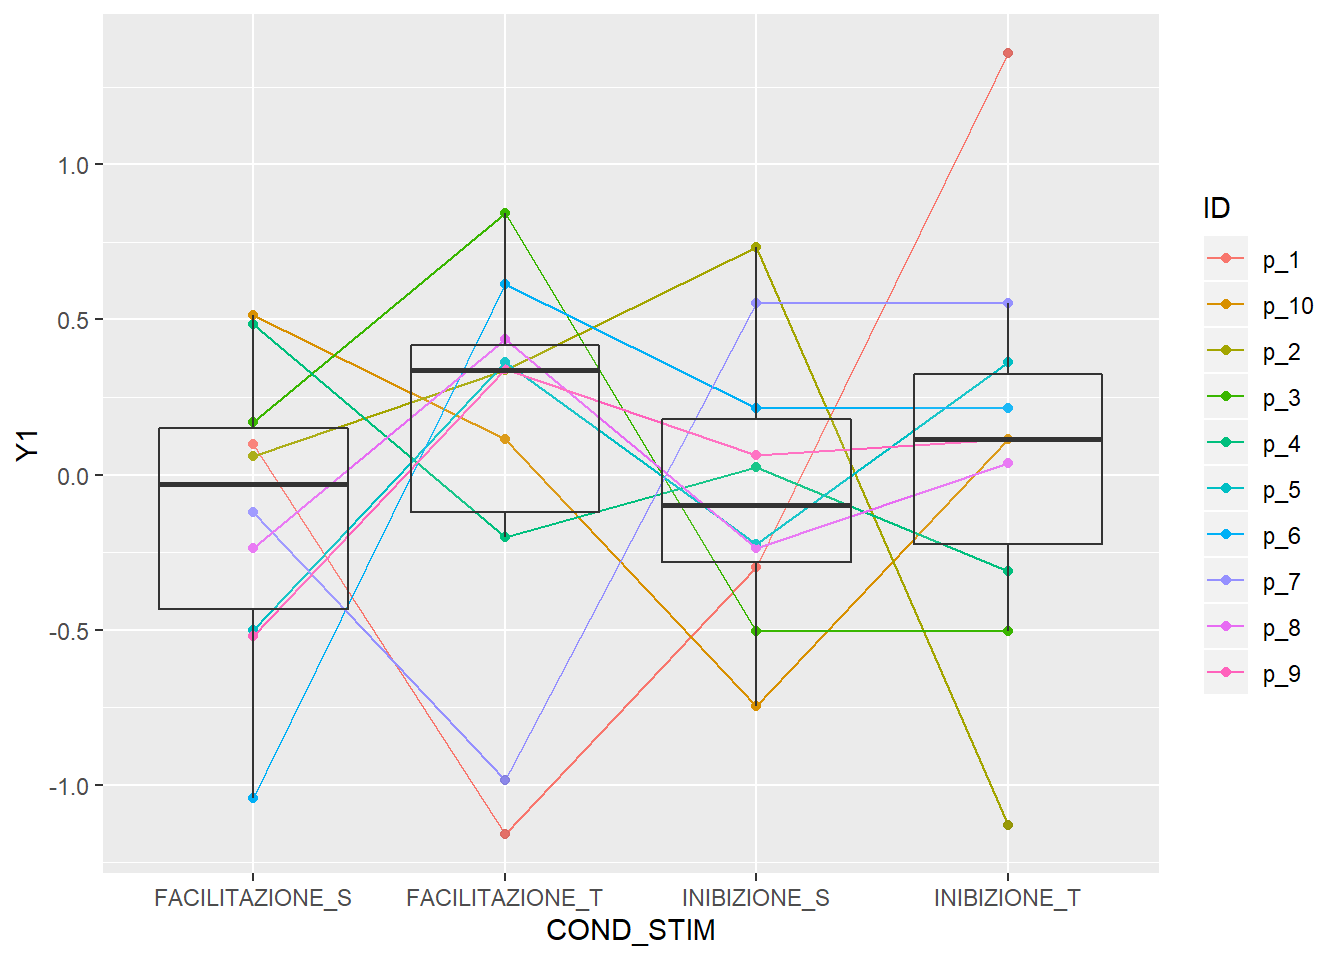
\includegraphics[width=500]{fMRI_multiple_testing_RandomFieldTheory_files/figure-latex/unnamed-chunk-4-1} \end{center}

\subsection{A toy example}\label{a-toy-example}

\begin{center}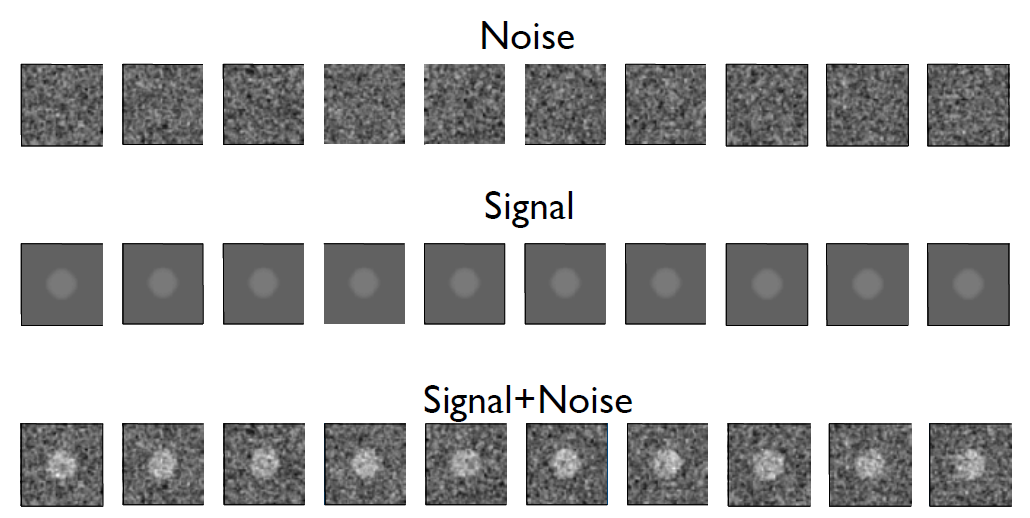
\includegraphics[width=700px]{./figs/sim_es} \end{center}

\begin{center}\rule{0.5\linewidth}{\linethickness}\end{center}

\begin{center}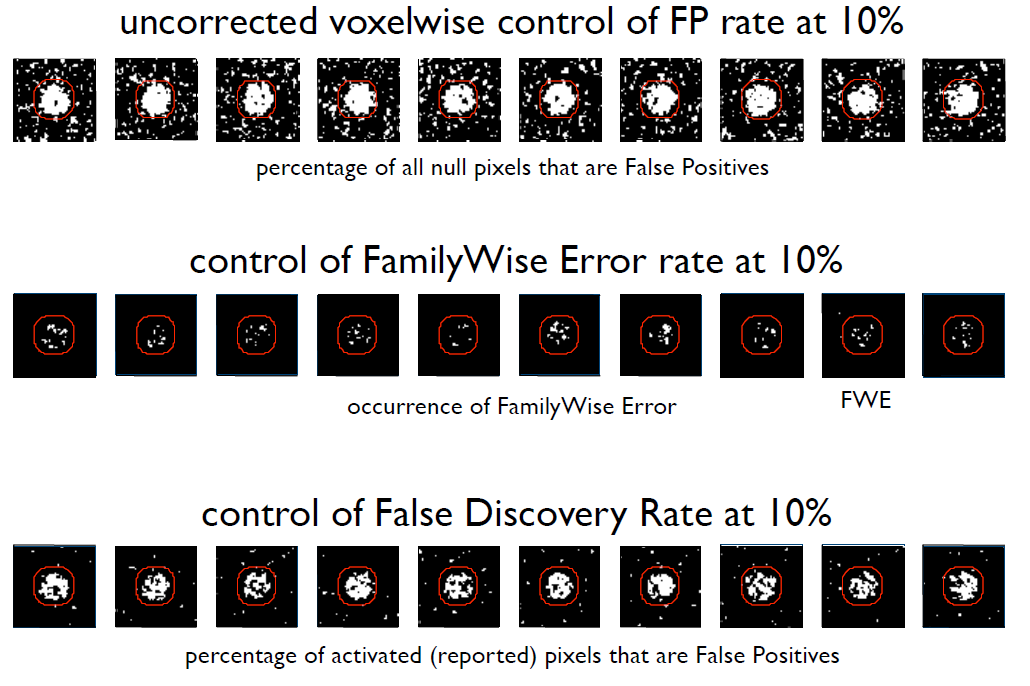
\includegraphics[width=700px]{./figs/sim_es2} \end{center}

\subsection{FDR with Dependent tests}\label{fdr-with-dependent-tests}

BH is valid under assumption of independence between the p-value and
\textbf{Positive Regression Dependency} on each subset of true null
hypos\\
(eg normal with positive correlation)

Usually valid in fMRI data

For ANY dependence: \textbf{BY}

\emph{Benjamini Y, Yekutieli D. (2001) The control of the false
discovery rate in multiple testing under dependency. Annals of
statistics 29 (4): 1165-1188}

But usually very conservative (sometime more than Bonferroni)

\subsection{FWER or FDR?}\label{fwer-or-fdr}

\textbf{Assumptions implied by FDR}\\
The assumptions are exchangeable:\\
True Rejections can compensate False Rejections

I don't think that the FDR is adequate in fMRI data.

\textbf{Problems} - Cheating - Subsets

\begin{center}\rule{0.5\linewidth}{\linethickness}\end{center}

\textbf{Cheating} I can add not interesting hypotheses with significant
with p-values to compensate false rejections.

\textbf{Subsets}\\
FDR control does NOT imply control of FDR in all subsets\\
eg: I correct all the tests, while discussing only those that I know how
to better explain.

\begin{itemize}
\tightlist
\item
  FDR control on all subsets = FWER control
\item
  FWER control on all subsets = FWER control
\end{itemize}

\emph{Finner H, Roters M. (2001) On the false discovery rate and
expected type I errors. biometrical Journal\}; 43 (8): 985-1005}

\subsection{Subsets of Rejections}\label{subsets-of-rejections}

\begin{center}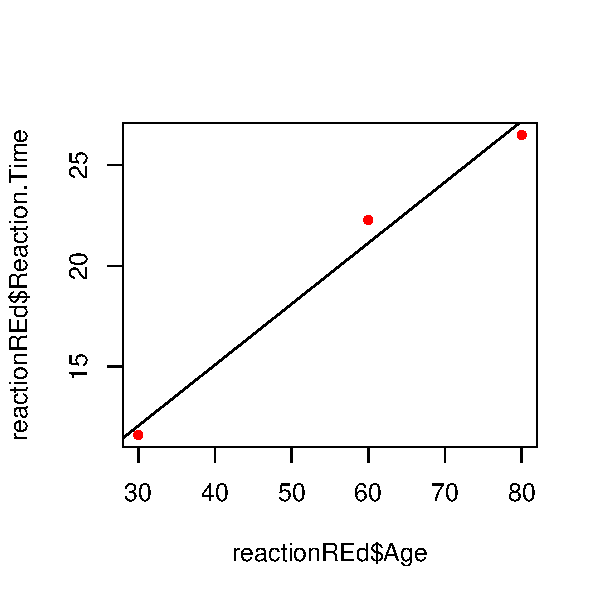
\includegraphics[width=700px]{fMRI_multiple_testing_RandomFieldTheory_files/figure-latex/unnamed-chunk-7-1} \end{center}

\section{Three levels of inference in
neuroscience}\label{three-levels-of-inference-in-neuroscience}

\subsection{Levels of inference}\label{levels-of-inference}

-- Voxel-level\\
-- Cluster-level\\
-- Set-level

\subsection{Voxel-level Inference}\label{voxel-level-inference}

\begin{center}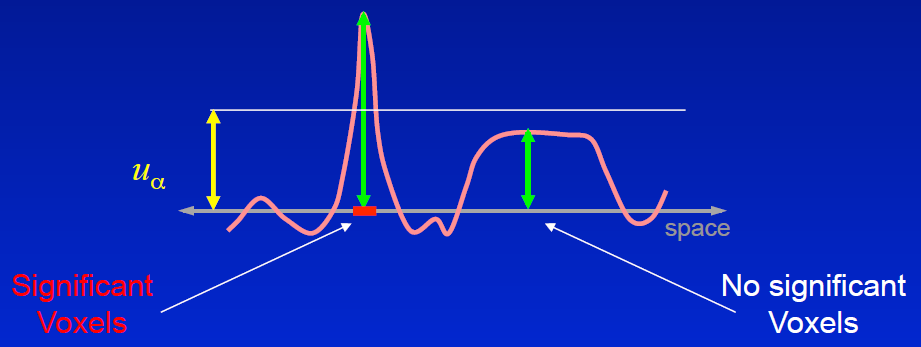
\includegraphics[width=700px]{./figs/voxel_level} \end{center}

\begin{itemize}
\tightlist
\item
  Retain voxels above \(\alpha\)-level threshold \(u_\alpha\)
\item
  Gives best spatial specificity:

  \begin{itemize}
  \tightlist
  \item
    The null hyp. at a single voxel can be rejected
  \end{itemize}
\end{itemize}

\subsection{Cluster-level Inference}\label{cluster-level-inference}

\begin{center}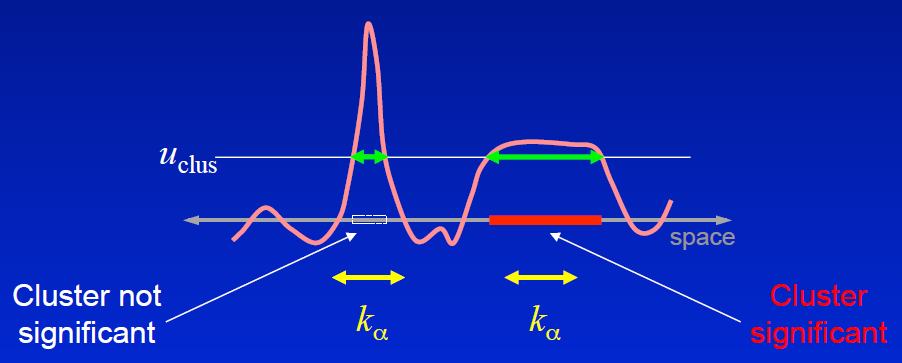
\includegraphics[width=700px]{./figs/cluster_level} \end{center}

\begin{itemize}
\item
  Typically better sensitivity
\item
  Worse spatial specificity

  -- The null hypo of entire cluster is rejected -- Only means that AT
  LEAST ONE voxels in cluster active
\end{itemize}

\subsection{Set-level Inference}\label{set-level-inference}

\begin{itemize}
\tightlist
\item
  Count number of blobs \(c\)

  \begin{itemize}
  \tightlist
  \item
    Minimum blob size \(k\)
  \end{itemize}
\item
  Worst spatial specificity

  \begin{itemize}
  \tightlist
  \item
    Only can reject global null hypothesis
  \item
    just a global inference, same as weak control
  \end{itemize}
\end{itemize}

\section{Voxel-level Inference}\label{voxel-level-inference-1}

\subsection{Do you Bonferroni\ldots{} or
not?}\label{do-you-bonferroni-or-not}

As we know, we test each hypothesis (voxel) at level:
\(\widetilde{\alpha} = \alpha/m\)

In fMRI, we use more often \(t\)-threshold (or \(z\)-threshold,
\(F\)-threshold, \(\chi^2\)-threshold -- similar results hold) instead
of \(p\)-values and \(\alpha\).

\(p\leq \widetilde{\alpha}\) Equivalent to
\(t\geq t_{1-\widetilde{\alpha}}\)

We look for the distribution of \(Max-T\) (maximum t-statistic for \(m\)
test under \(H_0\)).

\subsection{Smoothed Images -
Autocorrelation}\label{smoothed-images---autocorrelation}

\begin{center}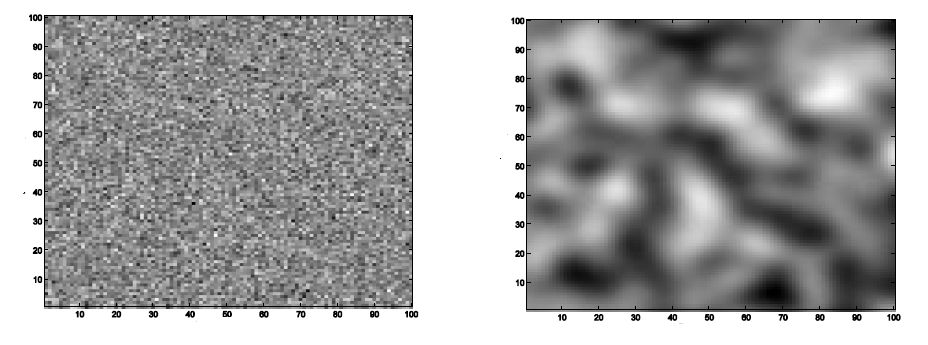
\includegraphics[width=700px]{./figs/indep_vs_smoothed} \end{center}

\begin{center}\rule{0.5\linewidth}{\linethickness}\end{center}

\textbf{Intrinsic smoothness}\\
-- MRI signals are aquired in k-space (Fourier space); after projection
on anatomical space, signals have continuous support\\
- Diffusion of vasodilatory molecules has extended spatial support

\textbf{Extrinsic smoothness}\\
-- Re-sampling during preprocessing\\
-- Deliberate additional smoothing to increase SNR\\
-- Robustness to between-subject anatomical differences

Unfortunately, the spatial correlation makes Bonferroni correction too
conservative

\subsection{RESEL}\label{resel}

\textbf{RESEL} stands for \textbf{RES}olution \textbf{EL}ement

A RESEL is simply a block of pixels that is the same size as the FWHM.

Eg: 10 voxels, 2.5 FWHM, 4 RESELS

\begin{center}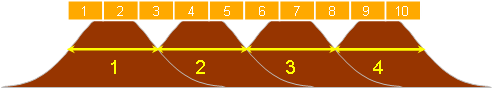
\includegraphics[width=600px]{./figs/resel_es} \end{center}

\begin{itemize}
\tightlist
\item
  Number of RESELS is similar to, but NOT equal to, the number of
  independent observations in an image
\item
  The number of resels depends only on the number of pixels, and the
  FWHM
\item
  Smoothness (FWHM) can be estimated from standardized residuals.
\end{itemize}

\subsection{Max-T distribution}\label{max-t-distribution}

We know there is some function of the number of Resels, \(R\), that
describes the Max-t distribution

We don't know how to calculate it

But there is an approximation of the tail, and that is what matters.

This approximation is derived from Random Field Theory (RFT) Theory

\subsection{Random Field Theory}\label{random-field-theory}

\begin{center}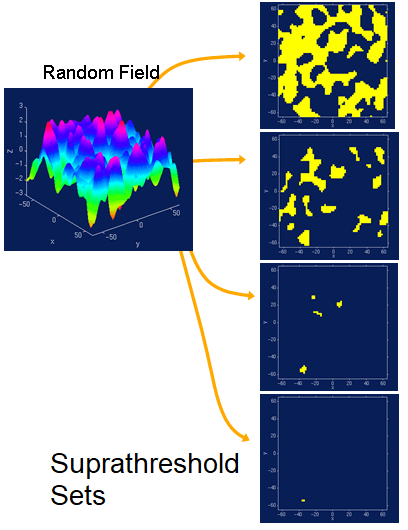
\includegraphics[width=400px]{./figs/RFT_supraThreshold} \end{center}

\begin{center}\rule{0.5\linewidth}{\linethickness}\end{center}

\textbf{Euler Characteristic \(\chi_u\) } can be thought of as the
number of blobs in an image after thresholding.

-- Topological Measure: \#blobs - \#holes\\
-- At high thresholds, just counts blobs \[
\begin{aligned}
  FWER &= P(Max-t\geq u\ |\ H_0)\\
       &= P(One\ or\ more\ blobs\ |H_0)\\
  (no\ holes) &\approx P(\chi_u\geq 1|H_0)\\
       &\leq E(\chi_u|H_0)
\end{aligned}
\]

e.g.~for Gaussian test statistic (i.e. \(z\), not \(t\)):
\[E(\chi_u|H_0)\approx R 2\pi^{-2}W^{-3} u^{2} exp(-u^2/2)\]

\(R\) is the number of resels, \(u\) is the z-score threshold

\subsection{How it works}\label{how-it-works}

\begin{itemize}
\tightlist
\item
  First we estimate the smoothness (spatial correlation) of our
  statistical map.
\item
  Then we use the smoothness values in the appropriate RFT equation, to
  give the expected EC at different thresholds.
\item
  This allows us to calculate the threshold \(u\) at which we would
  expect 5\% of equivalent statistical maps arising under the null
  hypothesis to contain at least one area above threshold.
\item
  All hypos (voxels) with \(t\geq u\) are rejected and FWER is
  controlled.
\end{itemize}

\section{Cluster-level inference}\label{cluster-level-inference-1}

\subsection{Spatial extent -
motivation}\label{spatial-extent---motivation}

\textbf{Peak extent} (voxel-level)

We see a t-value of 10. It is so surprising (under the null hypothesis)
that we have to reject it (i.e. \(t\)-statistic larger than
\(u_\alpha\)).

\textbf{Spatial extent} (cluster-level)

We threshold the t-map at \(u_{clust}=2.3\) (arbitrary threshold) and
look at the spatial extent of clusters.

We see 300 connected voxels all with t-values \(\geq u_{clust}=2.3\).

It is so surprising (under the null hypothesis) that we have to reject
it (i.e.~size of the cluster larger than \(k_\alpha\)).

\subsection{Cluster-level Inference}\label{cluster-level-inference-2}

Two step-process:\\
-- Define clusters by arbitrary threshold \(u_{clus}\)\\
-- Retain clusters larger than \(\alpha\)-level threshold \(k_\alpha\)

\begin{center}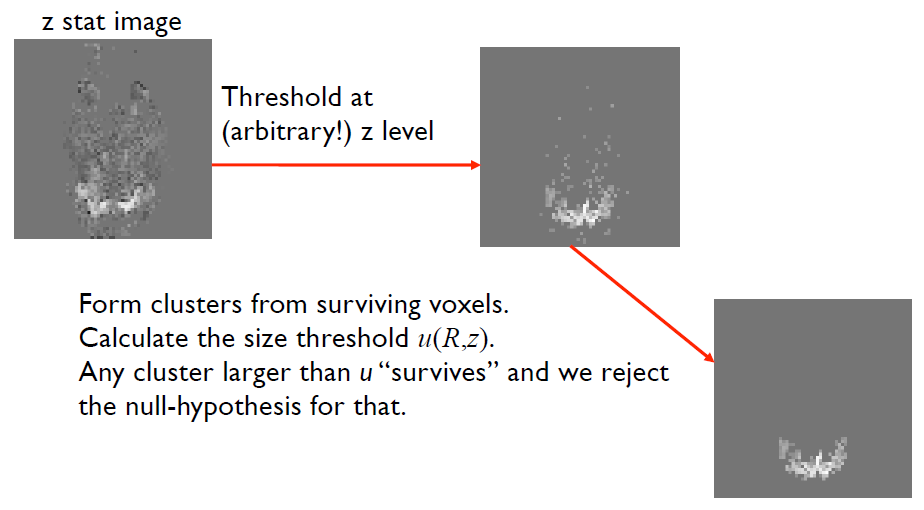
\includegraphics[width=700px]{./figs/clust_cookbook} \end{center}

\begin{center}\rule{0.5\linewidth}{\linethickness}\end{center}

If we reject any cluster we will reject the largest.

We need the distribution of the largest cluster (given a threshold
\(u_{clust}\)), under the null-hypothesis.

\(k_\alpha\) is the \((1-\alpha)\)-quantile of this distribution.

So, just as was the case for the \(t\)-values, we now have a
distribution \(f(R,u_{clust})\) that allows us to calculate a Family
Wise threshold \(k_\alpha\) pertaining to cluster size.

\begin{center}\rule{0.5\linewidth}{\linethickness}\end{center}

\(W=|\Lambda|^{-1/(2D)}=FWHM (4 log_e 2)^{-1/2}\), where
\(FWHM=FWHM_xFWHM_yFWHM_z\), \(\Lambda\) is the covariance matrix of the
field's first partial derivatives and \(D\) is the number of dimensions
(i.e. \(D=3\))

At high thresholds, the number of clusters \(\chi_u\) approximates the
number of maxima and has been shown to have a Poisson distribution
(Adler, 1981, Theorem 6.9.3, page 161):
\[ P(\chi_u = c) \approx \lambda(c, E(\chi_u))\]

\begin{itemize}
\item
  the expected number of maxima \(E(\chi_u)\) (i.e., clusters) is:
  \[E(\chi_u)\approx R 2\pi^{-(D+1)/2}W^{-D} u_{clust}^{D-1} exp(-u_{clust}^2/2)\]
\item
  Distribution of the number of voxels \(n\) in a cluster:\\
  \[P(n \geq k) \approx exp (-\beta k^{2/D})\], where
  \(\beta = [\Gamma(D/2 + 1)E(\chi)/(S \Phi(-u))]^{2/D}\)
\end{itemize}

\begin{center}\rule{0.5\linewidth}{\linethickness}\end{center}

The probability to observe a cluster with \(k\) or more voxles is

\[P(u_{clust}, k) \approx 1 - exp (-E(\chi)P(n \geq k))\] \(k_\alpha\)
is the \(k\) such that \(P(u_{clust}, k)=\alpha\).

\begin{center}\rule{0.5\linewidth}{\linethickness}\end{center}

\(k_\alpha\) depends on the initial \emph{cluster-forming} threshold
\(u_{clust}\).

\begin{center}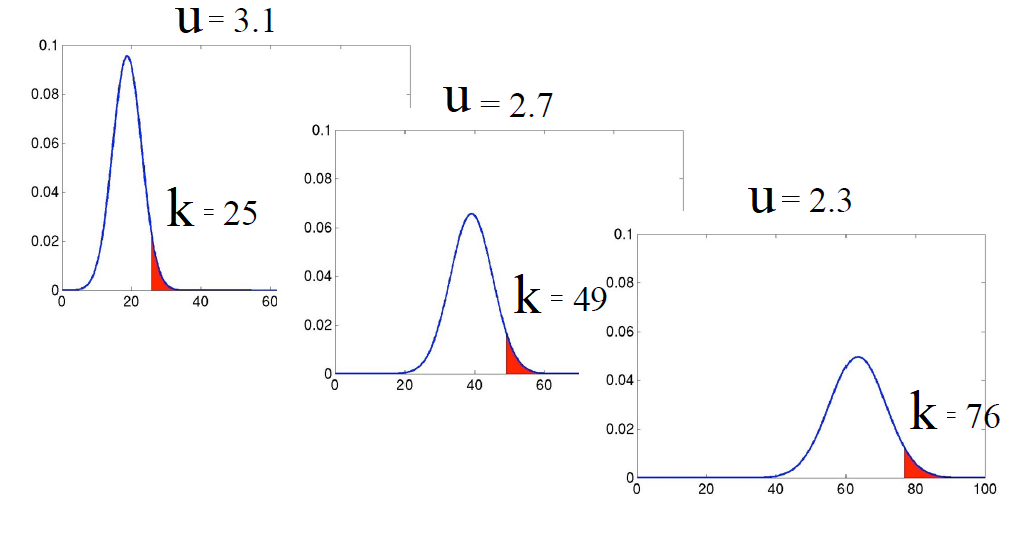
\includegraphics[width=700px]{./figs/RFT_Threshold_function} \end{center}

\subsection{Voxel/Cluster-level in a
glance}\label{voxelcluster-level-in-a-glance}

\begin{center}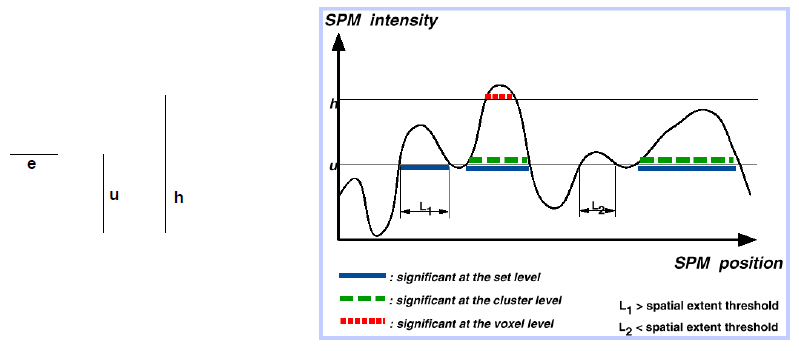
\includegraphics[width=700px]{./figs/spatial_extent} \end{center}

\subsection{Remarks}\label{remarks}

\begin{itemize}
\tightlist
\item
  Needs a null-hypothesis, a test-statistic and an initial cluster
  forming threshold.
\item
  Calculates a (size) threshold based on number of RESELS and initial
  (z) threshold
\end{itemize}

\textbf{Pros}

\begin{itemize}
\tightlist
\item
  Gives a (size) threshold such that the family-wise error is
  controlled.
\item
  Calculates that threshold very fast.
\end{itemize}

\subsection{Limitations}\label{limitations}

\textbf{Limitations (1/2)}

\begin{itemize}
\tightlist
\item
  \emph{Sufficient smoothness}

  \begin{itemize}
  \tightlist
  \item
    FWHM smoothness \(3-4\times\) voxel size (Z)\\
  \item
    More like \(\sim 10\times\) for low-df T images
  \end{itemize}
\item
  \emph{Smoothness estimate} is biased when images not sufficiently
  smooth
\item
  \emph{Multivariate normality}: virtually impossible to check
\item
  Several layers of \emph{approximations} (e.g.~Lattice Image Data
  \(\approx\) Continuous Random Field)
\item
  \emph{Stationarity} required for cluster size results
\end{itemize}

This can be solved via permutation-approach

\begin{center}\rule{0.5\linewidth}{\linethickness}\end{center}

\textbf{Limitations (2/2)}

\begin{itemize}
\tightlist
\item
  Inference pertains to entire cluster (i.e.~there is at least one
  voxel)

  \begin{itemize}
  \tightlist
  \item
    This can be solved via All-Resolution Inference approach
  \end{itemize}
\item
  Initial threshold is arbitrary and must be chosen a priori

  \begin{itemize}
  \tightlist
  \item
    This can be solved via All-Resolution Inference approach
  \end{itemize}
\end{itemize}

\ldots{} \textbf{A serious problem}, no jockes:\\
Eklund, Nicholsd and Knutsson (2016) Cluster failure: Why fMRI
inferences for spatial extent have inflated false-positive rates. PNAS

(permutation and All-Resolution Inference are the subject of the next
classes)


\end{document}
